% Copyright 2020 by Robert Hildebrand
%This work is licensed under a
%Creative Commons Attribution-ShareAlike 4.0 International License (CC BY-SA 4.0)
%See http://creativecommons.org/licenses/by-sa/4.0/

\chapter{Modeling: Linear Programming}

\begin{outcome}
\begin{enumerate}
\item Define what a linear program is
\item Understand how to model a linear program
\item View many examples and get a sense of what types of problems can be modeled as linear programs.
\end{enumerate}
\end{outcome}
\begin{resource}
\begin{itemize}
\item \href{https://www.youtube.com/watch?v=K7TL5NMlKIk&ab_channel=Dr.TreforBazett}{Youtube! - Modeling with Linear Programming - Watch 0:00 - 4:19}
\item \href{https://www.youtube.com/watch?v=E72DWgKP_1Y&t=1014s&ab_channel=TomS}{Youtube! - Watch 0:00 - 1:43}
\end{itemize}
\end{resource}

\begin{tryit}
\vizlink{modeling-intro}{From Words to Math}: a step-by-step interactive modeling tutorial.
\end{tryit}


Linear Programming, also known as Linear Optimization, is the starting point for most forms of optimization.  It is the problem of optimizing a linear function over linear constraints.   

In this chapter, we will define what this means, how to set up a linear program, and discuss many examples.   Examples will be connected with code in Excel and Python (using PuLP or Gurobipy modeling tools) so that you can easily start solving optimization problems.   Tutorials on these tools will come in later chapters.

As a warm-up, consider the following word problem.\\
\noindent \textbf{Question:} A movie theater sells adult tickets for $\$10$ each and child tickets for $\$6$ each. On Saturday, the theater sold $120$ tickets total and collected $\$1{,}000$ in ticket sales. How many adult and child tickets were sold?

\smallskip

\noindent \textbf{\textcolor{blue}{Solution:}} Let $x$ and $y$ denote the number of adult and child tickets sold, respectively. Then
\[
x + y = 120 \tag{1}
\]
\[
10x + 6y = 1{,}000. \tag{2}
\]
Substituting $x = 120 - y$ from (1) into (2) gives $10(120-y) + 6y = 1{,}000$, which simplifies to $4y = 200$, so $y = 50$ and $x = 70$.

\smallskip

In optimization, we follow a similar process of assigning variables and writing mathematical expressions from a word problem. However, instead of equations that pin down a unique answer, we typically have \emph{inequalities} that bound the variables in different ways, and an \emph{objective function} we wish to maximize or minimize. Thus, there can be many feasible solutions, and the goal is to find the best one.

\section{Introductory LP Example}
\label{sec:lp-intro-example}
We begin with a simple example.
\begin{examplewithallcode}{Screen Printing Shop}%
{https://github.com/open-optimization/open-optimization-or-examples/blob/master/linear-programming/screen_printing/screen_printing.xlsx}%
{https://github.com/open-optimization/open-optimization-or-examples/blob/master/linear-programming/screen_printing/screen_printing_pulp.ipynb}%
{https://github.com/open-optimization/open-optimization-or-examples/blob/master/linear-programming/screen_printing/screen_printing_gurobipy.ipynb}
%
A screen printing shop prints custom t-shirts and tote bags and must decide how many of each to make this week. Here is what the owner knows. On the revenue side, t-shirts sell for $\$15$ against $\$5$ of materials, and tote bags sell for $\$12$ against $\$4$ of materials. On the production side, two resources are scarce: the printing press (at most $150$ hours this week) and the drying/packaging station (at most $60$ hours). A t-shirt occupies the press for $2$ hours and a tote bag for $3$; each item then spends $1$ hour in drying and packaging. One more piece of information limits the plan: local demand for t-shirts tops out around $45$ per week, so making more than that would be wasted effort. What production plan earns the most profit?

To turn this story into mathematics, we need decision variables, an objective, and constraints. The decisions are the production quantities: let $x_1$ be the number of t-shirts and $x_2$ the number of tote bags made this week. Since each t-shirt nets $\$15 - \$5 = \$10$ and each tote bag nets $\$12 - \$4 = \$8$, the quantity the owner wants to maximize is the weekly profit:
\begin{equation}
z(x_1,x_2) = 10x_1 + 8x_2
\end{equation}
Next, each scarce resource becomes an inequality. Printing $x_1$ shirts and $x_2$ totes ties up $2x_1 + 3x_2$ press hours, which cannot exceed the $150$ available:
\begin{equation}
2x_1 + 3x_2 \leq 150
\end{equation}
The drying and packaging station tells the same kind of story, one hour per item against a $60$-hour budget:
\begin{equation}
x_1 + x_2 \leq 60
\end{equation}
The demand ceiling is the simplest constraint of all: $x_1 \leq 45$. Assembling the objective and the constraints, and remembering that production cannot be negative, gives the complete linear program:
\begin{equation}
\begin{aligned}
\max\;\;&& z(x_1,x_2) = 10x_1 + 8x_2\\
\st\;\;&&  2x_1 + 3x_2 &\leq 150\\
&& x_1 + x_2 &\leq 60\\
&& x_1 &\leq 45\\
&& x_1 &\geq 0\\
&& x_2 &\geq 0
\end{aligned}
\label{eqn:ScreenPrintEx}
\end{equation}
\label{ex:ScreenPrint}
\end{examplewithallcode}

\section{Modeling and Assumptions in Linear Programming}
\label{sec:lp-modeling-assumptions}

\begin{outcome}
\begin{enumerate}
\item Address key assumptions when choosing to model a problem with linear programming.
\end{enumerate}
\end{outcome}

\paragraph{A Generic Linear Program (LP)}

Linear programming (LP) is a mathematical optimization framework widely used in decision-making and resource allocation. In its most basic form, an LP seeks to optimize (maximize or minimize) a linear objective function subject to a set of linear constraints. These constraints typically represent limitations or requirements in real-world scenarios, such as budgets, capacities, or resource availability.

\smallskip \modelhead{Variables}\\
The decision variables represent the quantities we want to determine. For example:
\begin{itemize}
    \item $x_i$: Continuous variables ($x_i \in \mathbb{R}$, i.e., a real number), $\forall i = 1,\dots,n$.
\end{itemize}
These variables could represent amounts of products to produce, resources to allocate, or investments to make.  We can use any letters to represent these variables.  Typically we use $x_i$, but frequently will use $y_i$ or other letters depending on the context and what makes reading the problem most convenient.

\smallskip \modelhead{Parameters}\\
Parameters are the given data in the problem, which are assumed to be known in advance:
\begin{itemize}
    \item $c_i$: Cost coefficients for each decision variable, $\forall i = 1,\dots,n$. These values represent the contribution of each variable to the objective function.
    \item $a_{ij}$: Constraint coefficients, $\forall i = 1,\dots,n$ and $j = 1,\dots,m$. These define the relationships between decision variables and the constraints.
    \item $b_j$: Right-hand side values of the constraints, $\forall j = 1,\dots,m$. These represent limits or requirements for each constraint.
\end{itemize}

The general form of a linear program can be written as follows:

\begin{equation}
\begin{aligned}
\max\;\;&& z = c_1x_1 + \dots + c_nx_n \\
\st\;\;&& a_{11}x_1 + \dots + a_{1n}x_n &\leq b_1 \\
&& \hspace*{0.5in}\vdots \\
&& a_{m1}x_1 + \dots + a_{mn}x_n &\leq b_m \\
&& x_i &\geq 0 \quad \forall i=1, \dots, n.
\end{aligned}
\label{eqn:GeneralLPMax}
\end{equation}

\paragraph{Features of a Linear Program}

\begin{itemize}
    \item \textbf{Objective Function}: The linear function $z = c_1x_1 + \dots + c_nx_n$ represents the goal to optimize. This could involve maximizing profit, minimizing cost, or achieving some other measurable outcome.
    \item \textbf{Constraints}: The system of inequalities (or equalities) restricts the values of the decision variables. Each constraint reflects a real-world limitation, such as resource availability or capacity limits.
    \item \textbf{Feasibility}: The set of all possible solutions that satisfy the constraints is called the feasible region. The optimal solution must lie within this region.
    \item \textbf{Linear Relationships}: Both the objective function and constraints are linear, meaning the relationships between variables are additive and proportional.
    \item \textbf{Sets}: For specific optimization problems, it can be useful to define sets of variables or parameters to help write down the problem in a generic formulation.
\end{itemize}

\paragraph{Example of a Linear Program}

To illustrate, consider a specific example with three decision variables and four constraints, including a mix of constraint types ($\leq$, $\geq$, and $=$):

\smallskip \modelhead{Variables}\\
$x_i$: Continuous variables ($x_i \in \mathbb{R}$, i.e., a real number), $\forall i = 1,\dots,3$.

\smallskip \modelhead{Parameters}\\
\begin{itemize}
    \item $c_i$: Cost coefficients, $\forall i = 1,\dots,3$.
    \item $a_{ij}$: Constraint coefficients, $\forall i = 1,\dots,3$ and $j = 1,\dots,4$.
    \item $b_j$: Right-hand side values for each constraint, $\forall j = 1,\dots,4$.
\end{itemize}

\smallskip \modelhead{Model}
\begin{align*}
\min \quad & z = c_1x_1 + c_2x_2 + c_3x_3 \\
\st        & a_{11}x_1 + a_{12}x_2 + a_{13}x_3 \geq b_1 \\
& a_{21}x_1 + a_{22}x_2 + a_{23}x_3 \leq b_2 \\
& a_{31}x_1 + a_{32}x_2 + a_{33}x_3 = b_3 \\
& a_{41}x_1 + a_{42}x_2 + a_{43}x_3 \geq b_4 \\
& x_1 \geq 0, \; x_2 \leq 0, \; x_3 \text{ unrestricted.}
\end{align*}

A key feature of linear programming is the use of linear functions, defined as follows:

\begin{definition}{Linear Function}\label{def:linearfunction}
A function $z: \mathbb{R}^n \rightarrow \mathbb{R}$ is \textit{linear} if there are constants $c_1, \dots, c_n \in \mathbb{R}$ such that:
\begin{equation}
z(x_1, \dots, x_n) = c_1x_1 + \dots + c_nx_n.
\end{equation}
\label{def:LinearFunc}
\end{definition}

Linear functions are characterized by their simplicity and additivity, making them well-suited for optimization problems where proportionality is assumed. This simplicity allows linear programs to be solved efficiently, even for large-scale problems.

\subsection{Assumptions}
\label{sec:lp-assumptions}
When we wrote down the model in Example \ref{ex:ScreenPrint}, we quietly made four modeling assumptions.  They are worth stating out loud, because they tell you when a linear program is the right tool and when it is not.

\begin{description}
\item[Proportionality] Doubling a variable doubles its effect.  If one t-shirt earns \$8 and consumes 15 minutes of press time, then 50 shirts earn \$400 and consume 750 minutes.  No quantity discounts, no economies of scale, no setup costs: every unit behaves like the first one.

\item[Additivity] Effects add up across variables, with no interactions.  The press time used by t-shirts and the press time used by posters simply sum; producing one product does not make another product cheaper, more profitable, or harder to make.

\item[Divisibility] Variables may take fractional values.  The model is allowed to recommend printing half a shirt, whether or not that makes physical sense.

\item[Certainty] Every number in the model (the profit per shirt, the minutes per press run, the hours available) is treated as known exactly, not as an estimate or a random quantity.
\end{description}

Proportionality and additivity together say exactly that the objective and constraint functions are \emph{linear} in the sense of Definition~\ref{def:linearfunction}.  If your problem has quantity discounts, interaction effects, or fixed setup charges, a plain linear program does not capture it, though we will see in the integer programming chapters that some of these features can be recovered with clever modeling.

Divisibility deserves a closer look.  Some quantities divide naturally: ounces of ink, hours of labor, dollars of budget.  Items like t-shirts do not; nobody sells six tenths of a shirt.  In practice this matters less than it first appears.  When production quantities are large, an optimal plan calling for, say, several hundred shirts plus a fraction can be rounded to whole units with only a tiny effect on profit.  When whole-number answers truly matter, we add the integrality requirement explicitly, and the model becomes an \emph{integer program}, the subject of Part~\ref{part:IntroIntegerProgramming} of this book.

Certainty is the assumption most often violated in the real world: demand forecasts miss, prices move, machines run slow.  Fields such as \emph{stochastic programming} and \emph{robust optimization} extend linear programming to handle uncertain data, and sensitivity analysis (Chapter~\ref{ch:sensitivity}) lets us ask how much the data could change before our optimal plan changes.  For now, we take the data as given.

\begin{learningcheckpoint}[label={lc:lp-assumptions}]
In a short sentence or two, discuss whether the problem in
Example~\ref{ex:ScreenPrint} meets all assumptions of a linear programming model.
%Do the same for Exercise~\autoref{ex:ChemicalPlant}.

\emph{Hint: Can you print $\tfrac{2}{3}$ of a t-shirt? Can you run a process
for $\tfrac{1}{3}$ of an hour?}
\end{learningcheckpoint}

\section{Examples}
\label{sec:lp-examples}

\begin{outcome}

\begin{enumerate}
\item Identify decision variables and parameters
\item Learn how to format a linear optimization problem.
\item Identify and understand common classes of linear optimization problems.
\end{enumerate}
\end{outcome}

We will begin with a few examples, and then discuss specific problem types that occur often.

\begin{examplewithallcode}{Production Planning}
{https://github.com/open-optimization/open-optimization-or-book/blob/master/Intro-Math-Programming/baseText/optimization/optimization-examples/production-planning-excel.xlsx}
{https://github.com/open-optimization/open-optimization-or-book/tree/master/Intro-Math-Programming/baseText/optimization/optimization-examples/production_planning_pulp.ipynb}
{https://github.com/open-optimization/open-optimization-or-book/tree/master/Intro-Math-Programming/baseText/optimization/optimization-examples/production_planning_gurobi.ipynb}
\label{example:production-planning}
A manufacturing firm seeks to optimize its production schedule over a two-day planning horizon to meet daily demand while minimizing costs. The firm starts with an initial inventory of \( s_0 \) units. The costs associated with production and inventory are as follows:

\begin{itemize}
    \item \textbf{Production costs:} \$10 per unit on Day 1, and \$16 per unit on Day 2.
    \item \textbf{Inventory cost:} \$5 per unit for carrying excess inventory from one day to the next.
\end{itemize}

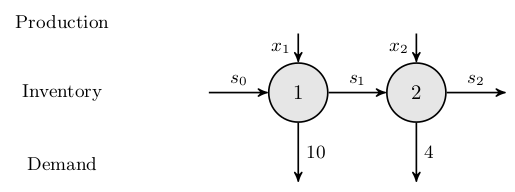
\includegraphics[width=0.85\linewidth]{figs/modeling-linear-programming-tikz01.png}

The goal is to determine the number of units to produce each day and the inventory levels to minimize total costs while satisfying the demand for each day.

\end{examplewithallcode}

\begin{solution}
 \modelhead{Sets}
\begin{itemize}
    \item Days of production $ = \{1, 2\}$.
\end{itemize}
 \modelhead{Parameters} 
\begin{itemize}
    \item $c_{p1}$: Per unit production cost on Day 1 (\$10).
    \item $c_{p2}$: Per unit production cost on Day 2 (\$16).
    \item $c_{inv}$: Per unit inventory cost (\$5).
    \item $d_1$: Demand on Day 1 (10 units).
    \item $d_2$: Demand on Day 2 (4 units).
        \item $s_0$: Inventory at the start of Day 1.
\end{itemize}

 \modelhead{Variables} 
\begin{itemize}
    \item $x_1$: Number of units produced on Day 1.
    \item $x_2$: Number of units produced on Day 2.
    \item $s_1$: Inventory at the end of Day 1.
    \item $s_2$: Inventory at the end of Day 2.
\end{itemize}

\modelhead{Model}
\begin{align*}
\min \quad & z = 10x_1 + 16x_2 + 5s_1 + 5s_2   \tag{Total cost} \\
\st        & s_0 + x_1 = 10 + s_1   \tag{Day 1 balance} \\
& s_1 + x_2 = 4 + s_2   \tag{Day 2 balance} \\
& x_1, x_2, s_0, s_1, s_2 \geq 0.   \tag{Non-negativity constraints}
\end{align*}

\end{solution}

\begin{definition}{Optimization model components}
When defining an optimization model, it is essential to identify and clearly articulate the following five components:

\begin{itemize}
    \item \textbf{Sets:} What lists of data do you need to write down? These could include indices, categories, or groups relevant to the problem.
    \item \textbf{Parameters (Data):} What is the actual data for the problem? These are the fixed numerical values such as costs, capacities, or resource availabilities.
    \item \textbf{Decision Variables:} What decisions need to be made to provide a solution? These variables represent the quantities that can be controlled or adjusted, such as production levels or resource allocations.
    \item \textbf{Objective Function:} The expression that we want to maximize or minimize. This is the goal of the optimization, such as minimizing cost or maximizing profit.
    \item \textbf{Constraints:} Certain rules that those decision variables should satisfy. These include limitations or requirements, such as resource capacities or demand fulfillment.
\end{itemize}

Each of these components plays a key role in formulating a well-structured optimization model that accurately represents the problem and provides actionable solutions.  The role of Sets will become more important as we get into more complicated optimization models.
\end{definition}

\newpage
\begin{examplewithallcode}{Bakery Production}
{https://github.com/open-optimization/open-optimization-or-book/blob/master/Intro-Math-Programming/baseText/optimization/optimization-examples/bakery-production-excel.xlsx}
{https://github.com/open-optimization/open-optimization-or-book/tree/master/Intro-Math-Programming/baseText/optimization/optimization-examples/bakery_production_pulp.ipynb}
{https://github.com/open-optimization/open-optimization-or-book/tree/master/Intro-Math-Programming/baseText/optimization/optimization-examples/bakery_production_gurobi.ipynb}
\label{example:bakery-production}
A small bakery produces three products each day: cakes, cookies, and muffins. Each item requires a specific amount of ingredients and baking time, and each contributes to the bakery’s profit. The bakery operates with daily limits on flour, sugar, and baking time due to ingredient supply and staffing constraints.

Each cake earns a profit of \$6.00, requires 500 grams of flour, 200 grams of sugar, and 60 minutes of baking time. Each cookie earns a profit of \$1.50, requires 100 grams of flour, 50 grams of sugar, and 10 minutes of baking time. Each muffin earns a profit of \$2.50, requires 200 grams of flour, 80 grams of sugar, and 20 minutes of baking time.

The bakery has at most 4,800 grams of flour, 2,060 grams of sugar, and 480 minutes of baking time available each day.

Determine how many cakes, cookies, and muffins the bakery should produce each day in order to maximize its total profit, while staying within the limits on flour, sugar, and baking time.

\subsection*{Linear Programming Model}

\[
\begin{aligned}
\text{Maximize} \quad & 6x_1 + 1.5x_2 + 2.5x_3 \\
\text{subject to} \quad
& 500x_1 + 100x_2 + 200x_3 \leq 4800 \quad \text{(Flour)} \\
& 200x_1 + 50x_2 + 80x_3 \leq 2060 \quad \text{(Sugar)} \\
& 60x_1 + 10x_2 + 20x_3 \leq 480 \quad \text{(Baking time)} \\
& x_1, x_2, x_3 \geq 0 \\
& x_1, x_2, x_3 \in \mathbb{Z} \quad \text{(if integer production is required)}
\end{aligned}
\]
\end{examplewithallcode}

\begin{examplewithallcode}{Production with welding robot}
{https://github.com/open-optimization/open-optimization-or-examples/blob/master/linear-programming/production_welding/production-welding-robot.xlsx}
{https://github.com/open-optimization/open-optimization-or-examples/blob/master/linear-programming/production_welding/production_welding_pulp.ipynb}
{https://github.com/open-optimization/open-optimization-or-examples/blob/master/linear-programming/production_welding/production_welding_gurobipy.ipynb}
%{productionproblem}{}{}{}
\label{example:welding-robot}
You have 21 units of transparent aluminum alloy (TAA), LazWeld1, a joining robot leased for 23 hours, and CrumCut1, a cutting robot leased for 17 hours of aluminum cutting. You also have production code for a bookcase, desk, and cabinet, along with commitments to buy any of these you can produce for \$18,  \$16, and  \$10 apiece, respectively.  A bookcase requires 2 units of TAA, 3 hours of joining, and 1 hour of cutting, a desk requires 2 units of TAA, 2 hours of joining, and 2 hours of cutting, and a cabinet requires 1 unit of TAA, 2 hours of joining, and 1 hour of cutting. 

Formulate an LP to maximize your revenue given your current resources.
\end{examplewithallcode}

\begin{solution}

\noindent\medskip \modelhead{Sets}
\begin{itemize}
\item The types of objects $ = \{$ bookcase,~desk,~cabinet$\}$.
\end{itemize}
\medskip \modelhead{Parameters} 
\begin{itemize}
\item Purchase cost of each object
\item Units of TAA needed for each object
\item Hours of joining needed for each object
\item Hours of cutting needed for each object
\item Hours of TAA, Joining, and Cutting available on robots
\end{itemize}

\noindent\medskip \modelhead{Variables} \\
$x_i$ : number of units of product $i$ to produce, \\
for all $ i = $bookcase,~desk,~cabinet.\\

\noindent \medskip \modelhead{Model}
\begin{align*}
\max \quad & z = 18x_1 + 16x_2 + 10x_3   \tag{profit} \\
\st        & 2x_1 + 2x_2 + 1x_3 \le 21   \tag{TAA} \\
& 3x_1 + 2x_2 + 2x_3 \le 23   \tag{LazWeld1} \\
& 1x_1 + 2x_2 + 1x_3 \le 17   \tag{CrumCut1} \\
& x_1, x_2, x_3 \ge 0.
\end{align*}
\end{solution}

\begin{examplewithallcode}{The Diet Problem}
{https://github.com/open-optimization/open-optimization-or-book/blob/master/Intro-Math-Programming/baseText/optimization/optimization-examples/diet-problem.xlsx}
{https://github.com/open-optimization/open-optimization-or-book/tree/master/Intro-Math-Programming/baseText/optimization/optimization-examples/diet_problem_pulp.ipynb}
{https://github.com/open-optimization/open-optimization-or-book/tree/master/Intro-Math-Programming/baseText/optimization/optimization-examples/diet_problem_gurobi.ipynb}
\label{example:diet-problem}

In the future (as envisioned in a bad 70's science fiction film) all food is in tablet form, and there are four types, green, blue, yellow, and red. A balanced, futuristic diet requires at least 20 units of Iron, 25 units of Vitamin B, 30 units of Vitamin C, and 15 units of Vitamin D. Formulate an LP that ensures a balanced diet at the minimum possible cost.
\end{examplewithallcode}

\begin{table}[h!]
\begin{center}
\label{tab:pillContent}
\begin{tabular}{|c|c|c|c|c|c|}
\hline
Tablet & Iron & B & C & D & Cost (\$) \\ \hline
Chem 1 & 6 & 6 & 7 & 4 & 1.25 \\
Chem 2 & 4 & 5 & 4 & 9 & 1.05 \\
Chem 3 & 5 & 2 & 5 & 6 & 0.85 \\
Chem 4 & 3 & 6 & 3 & 2 & 0.65 \\
\hline
\end{tabular}
\end{center}
\end{table}

\begin{solution}
\smallskip \modelhead{Sets}
\begin{itemize}
\item Set of tablets $\{1,2,3,4\}$
\end{itemize}

\smallskip \modelhead{Parameters}
\begin{itemize}
\item Iron in each tablet
\item Vitamin B in each tablet
\item Vitamin C in each tablet
\item Vitamin D in each tablet
\item Cost of each tablet
\end{itemize}

\smallskip  \modelhead{Variables} \\
$x_i$ : number of tablets of type $i$ to include in the diet, $\forall i \in \{1,2,3,4\}$.\\

\smallskip  \modelhead{Model}
\begin{align*}
\min \quad && z = 1.25x_1 + 1.05x_2 + 0.85x_3 + 0.65x_4 \\
\st \quad &&  6x_1 + 4x_2 + 5x_3 + 3x_4 &\ge 20  \\
&& 6x_1 + 5x_2 + 2x_3 + 6x_4 &\ge 25 \\
&& 7x_1 + 4x_2 + 5x_3 + 3x_4 &\ge 30 \\
&& 4x_1 + 9x_2 + 6x_3 + 2x_4 &\ge 15  \\
&& x_1, x_2, x_3, x_4 &\ge 0. 
\end{align*}
\end{solution}

%The optimal diet costs \$5.35, and consists of 4.0625 green tablets and 0.3125 blue tablets.

\begin{examplewithallcode}{The Next Diet Problem}
{https://github.com/open-optimization/open-optimization-or-book/blob/master/Intro-Math-Programming/baseText/optimization/optimization-examples/diet-problem-next.xlsx}
{https://github.com/open-optimization/open-optimization-or-book/tree/master/Intro-Math-Programming/baseText/optimization/optimization-examples/diet_problem_next_pulp.ipynb}
{https://github.com/open-optimization/open-optimization-or-book/tree/master/Intro-Math-Programming/baseText/optimization/optimization-examples/diet_problem_next_gurobi.ipynb}

Progress is important, and our last problem had too many tablets, so we are going to produce a single, purple, 10 gram tablet for our futuristic diet requirements, which are at least 20 units of Iron, 25 units of Vitamin B, 30 units of Vitamin C, and 15 units of Vitamin D, and 2000 calories. The tablet is made from blending 4 nutritious chemicals; the following table shows the units of our nutrients per, and cost of, grams of each chemical.

Formulate an LP that ensures a balanced diet at the minimum possible cost.
\end{examplewithallcode}

\begin{table}[h!] \begin{center} \begin{tabular} {|c|c|c|c|c|c|c|}
\hline Tablet  & Iron  &  B &  C &  D & Calories & Cost (\$) \\ \hline
\hline  Chem 1  & 6    & 6         & 7         & 4         &  1000    & 1.25 \\
\hline  Chem 2  & 4    & 5         & 4         & 9         &  250     & 1.05 \\
\hline  Chem 3  & 5    & 2         & 5         & 6         &  850     & 0.85 \\
\hline  Chem 4  & 3    & 6         & 3         & 2         &  750     & 0.65 \\
\hline
\end{tabular} \end{center} \end{table}

\begin{solution}

\smallskip \modelhead{Sets}
\begin{itemize}
\item Set of chemicals $\{1,2,3,4\}$
\end{itemize}
\smallskip \modelhead{Parameters}
\begin{itemize}
\item Iron in each chemical
\item Vitamin B in each chemical
\item Vitamin C in each chemical
\item Vitamin D in each chemical
\item Cost of each chemical
\end{itemize}
\smallskip \modelhead{Variables} \\
$x_i$ : grams of chemical $i$ to include in the purple tablet, $\forall i = 1,2,3,4$.\\
\smallskip \modelhead{Model}
\begin{align*}
\min\ && z = 1.25x_1 + 1.05x_2 + 0.85x_3 + 0.65x_4 \\
\st &&  6x_1 + 4x_2 + 5x_3 + 3x_4 &\ge 20 \\
&& 6x_1 + 5x_2 + 2x_3 + 6x_4 &\ge 25  \\
&& 7x_1 + 4x_2 + 5x_3 + 3x_4 &\ge 30  \\
&& 4x_1 + 9x_2 + 6x_3 + 2x_4 &\ge 15  \\
&& 1000x_1 + 250x_2 + 850x_3 + 750x_4 &\ge 2000 \\
&& x_1 + x_2 + x_3 + x_4 &= 10  \\
&& x_1, x_2, x_3, x_4 &\ge 0. 
\end{align*}

\end{solution}

The diet problem might feel like a toy.  It is not.

\begin{casestudybox}{Feeding Millions: The World Food Programme's Optimization Engine}
\label{case:wfp}

The United Nations World Food Programme (WFP) is the world's largest humanitarian organization, assisting roughly 100 million people a year in places like Iraq, Yemen, and South Sudan.  Every operation must answer the same questions: \emph{what} food basket to provide, \emph{where} to buy it, and \emph{how} to move it.  WFP built an optimization tool, Optimus, that answers all three at once, and the team won the 2021 INFORMS Franz Edelman Award for it.

\subsection*{The Challenge}
A food basket must meet nutritional requirements (energy, protein, fat, micronutrients) for a beneficiary, using commodities that can actually be procured and delivered through a network of suppliers, ports, warehouses, and distribution points, each with costs and capacities.  Cheaper baskets can be less nutritious; more nutritious baskets can be undeliverable.  Before Optimus, these decisions were made separately by different teams.

\subsection*{The Solution: The Diet Problem Meets Network Flow}
\textbf{Model type: mixed-integer linear program.  The core is the classical diet LP joined to a min-cost flow model; integer variables handle choices such as transfer modality (food vs.\ cash).  No machine learning inside the optimization; demand and price inputs come from WFP assessments.}

A simplified version with the two key ingredients:

\modelhead{Variables}
\begin{itemize}
\item Let $x_k \geq 0$ be the amount of commodity $k$ (grams per person per day) in the food basket.
\item Let $f_{ka} \geq 0$ be the flow of commodity $k$ on arc $a$ of the supply network.
\end{itemize}

\modelhead{Model}
\begin{align*}
\min \quad & \sum_{k} c^{\text{proc}}_k\, x_k + \sum_{k,\,a} c^{\text{transp}}_a\, f_{ka}   \tag{procurement + transport cost} \\
\st        & \sum_{k} n_{jk} \, x_k \geq R_j &&\quad \text{for each nutrient } j   \tag{nutritional requirements} \\
           & \text{flow conservation linking } f_{ka} \text{ to deliveries of } x_k   \tag{the basket must actually arrive} \\
           & \sum_{k} f_{ka} \leq u_a &&\quad \text{for each arc } a   \tag{port/route capacities} \\
           & x_k \geq 0, \quad f_{ka} \geq 0,
\end{align*}
where $n_{jk}$ is the amount of nutrient $j$ per gram of commodity $k$ and $R_j$ is the daily requirement.  The published model adds palatability rules (e.g., the basket cannot be all lentils), sourcing decisions, multi-period planning, and the food-vs.-cash modality choice, which is where the integer variables enter.

\subsection*{Assumptions and Simplifications}
\begin{itemize}
\item Nutritional needs are modeled per ``average beneficiary''; the paper discusses requirements by demographic profile.
\item Prices and lead times are taken as data; the paper describes how WFP updates them per operation.
\end{itemize}

\subsection*{Implementation and Results}
In Iraq, the tool cut operating costs by 17 percent, and the resulting food baskets met 98 percent of the nutrition requirements; WFP has since applied it across its major operations.  The full MILP is printed in the paper, which is open access, so students can read exactly what was modeled and what was assumed.

\subsection*{References}
\begin{itemize}
\item K. Peters, S. Silva, R. Gon$\c{c}$alves, M. Kavelj, H. Fleuren, D. den Hertog, O. Ergun, M. Freeman. ``The Nutritious Supply Chain: Optimizing Humanitarian Food Assistance.'' \emph{INFORMS Journal on Optimization} 3(2), 200--226, 2021. \url{https://doi.org/10.1287/ijoo.2019.0047}
\end{itemize}
\end{casestudybox}

\begin{examplewithallcode}{Work Scheduling Problem}
{https://github.com/open-optimization/open-optimization-or-book/blob/master/Intro-Math-Programming/baseText/optimization/optimization-examples/work_scheduling_excel.xlsx}
{https://github.com/open-optimization/open-optimization-or-book/tree/master/Intro-Math-Programming/baseText/optimization/optimization-examples/work_scheduling_pulp.ipynb}
{https://github.com/open-optimization/open-optimization-or-book/tree/master/Intro-Math-Programming/baseText/optimization/optimization-examples/work_scheduling_gurobi.ipynb}
\label{example:work-scheduling}

You are the manager of LP Burger. The following table shows the minimum number of employees required to staff the restaurant on each day of the week. Each employee must work for five consecutive days. Formulate an LP to find the minimum number of employees required to staff the restaurant.

\end{examplewithallcode}

\begin{table}[h!] \begin{center} \begin{tabular} {|l|l|} 
\hline Day of Week & Workers Required   \\ \hline
\hline  1 = Monday & 6  \\
\hline  2 = Tuesday & 4  \\
\hline  3 = Wednesday & 5  \\
\hline  4 = Thursday & 4  \\
\hline  5 = Friday & 3  \\
\hline  6 = Saturday & 7  \\
\hline  7 = Sunday & 7  \\
\hline \end{tabular} \end{center} \end{table}

\begin{solution} This problem has multiple optimal solutions for which days workers begin working on, all of which result in 8 total workers hired.

\modelhead{Variables} \\
$x_i$ : the number of workers that start 5 consecutive days of work on day $i$, $ i = 1,\dots,7$ \\
\smallskip \modelhead{Model}
\begin{align*}
\min \quad & z = x_1 + x_2 + x_3 + x_4 + x_5 + x_6 + x_7 \\
\st        & x_1 + x_4 + x_5 + x_6 + x_7 \ge 6   \tag{Mon} \\
& x_2 + x_5 + x_6 + x_7 + x_1 \ge 4   \tag{Tue} \\
& x_3 + x_6 + x_7 + x_1 + x_2 \ge 5   \tag{Wed} \\
& x_4 + x_7 + x_1 + x_2 + x_3 \ge 4   \tag{Thu} \\
& x_5 + x_1 + x_2 + x_3 + x_4 \ge 3   \tag{Fri} \\
& x_6 + x_2 + x_3 + x_4 + x_5 \ge 7   \tag{Sat} \\
& x_7 + x_3 + x_4 + x_5 + x_6 \ge 7   \tag{Sun} \\
& x_1, \dots, x_7 \ge 0.
\end{align*}

One solution is as follows. The LP relaxation gives $z_{LP} = 7.333$ with fractional values $(x_1, \dots, x_7) = (0,\; 0.333,\; 1,\; 2.333,\; 0,\; 3.333,\; 0.333)$. Rounding to an integer solution yields $z_{IP} = 8$ with $(x_1, \dots, x_7) = (0,\; 0,\; 0,\; 3,\; 0,\; 4,\; 1)$.
\end{solution}

\newpage
\begin{examplewithallcode}{LP Burger - extended}
{https://github.com/open-optimization/open-optimization-or-book/blob/master/Intro-Math-Programming/baseText/optimization/optimization-examples/work_scheduling_excel_extended.xlsx}
{https://github.com/open-optimization/open-optimization-or-book/blob/master/Intro-Math-Programming/baseText/optimization/optimization-examples/work_scheduling_extended_pulp.ipynb}
{https://github.com/open-optimization/open-optimization-or-book/blob/master/Intro-Math-Programming/baseText/optimization/optimization-examples/work_scheduling_gurobi.ipynb}
LP Burger has changed its policy, and allows, at most, two part-time workers, who work for two consecutive days in a week.  Formulate this problem.
\end{examplewithallcode}
\begin{solution}
\modelhead{Variables} \\
$x_i$ : the number of workers that start 5 consecutive days of work on day $i$, $ i = 1,\cdots,7$ \\
$y_i$ : the number of workers that start 2 consecutive days of work on day $i$, $ i = 1,\cdots,7$.

\smallskip \modelhead{Model}
\begin{align*}
\min \quad && z = 5(x_1 + x_2 + x_3 + x_4 + x_5 + x_6 + x_7) \\
&& + 2(y_1 + y_2 + y_3 + y_4 + y_5 + y_6 + y_7) \nonumber \\
\st \quad && x_1 + x_4 + x_5 + x_6 + x_7 + y_1 + y_7 &\ge 6 \\
&& x_2 + x_5 + x_6 + x_7 + x_1 + y_2 + y_1 &\ge 4 \\
&&           x_3 + x_6 + x_7 + x_1 + x_2 + y_3 + y_2 &\ge 5 \\
&&           x_4 + x_7 + x_1 + x_2 + x_3 + y_4 + y_3 &\ge 4 \\
&&           x_5 + x_1 + x_2 + x_3 + x_4 + y_5 + y_4 &\ge 3 \\
&&           x_6 + x_2 + x_3 + x_4 + x_5 + y_6 + y_5 &\ge 7 \\
&&           x_7 + x_3 + x_4 + x_5 + x_6 + y_7 + y_6 &\ge 7 \\
&&           y_1 + y_2 + y_3 + y_4 + y_5 + y_6 + y_7 &\le 2 \\
&&           x_i \ge 0, y_i \ge 0, \forall i = 1,\cdots,7.
\end{align*}
\end{solution}

% SUBSECTION 3.2.1
\newpage
\subsection{Knapsack Problem}
We consider now a simple example where the variables can only take the values of 0 or 1.  We call these \emph{binary variables}.
\begin{examplewithallcode}{Camping Trip}
{https://github.com/open-optimization/open-optimization-or-book/blob/master/Intro-Math-Programming/baseText/optimization/optimization-examples/knapsack-problem-excel.xlsx}
{https://github.com/open-optimization/open-optimization-or-book/tree/master/Intro-Math-Programming/baseText/optimization/optimization-examples/knapsack-three-two-one-gurobi.ipynb}
{https://github.com/open-optimization/open-optimization-or-book/tree/master/Intro-Math-Programming/baseText/optimization/optimization-examples/knapsack-three-two-one-pulp.ipynb}
Imagine you are preparing for a week-long camping trip to the mountains. You have a backpack with a weight capacity of 20 kilograms. Your goal is to pack the most valuable items to ensure a comfortable and safe trip without exceeding the backpack's weight limit. Each item has a weight and a value associated with it, representing its importance and utility for the trip. The table below lists the potential items you can take, their weights in kilograms, and their values on a scale from 1 to 10 (with 10 being the most valuable).
\newline
Formulate an Integer Program to find the optimal items you should bring on your trip with you. 
\end{examplewithallcode}

\begin{table}[h!] \begin{center} \begin{tabular} {|l|l|l|l|} 
\hline Item & Index & Weight (kg) & Value  \\ \hline
\hline Tent & A & 4 & 10  \\
\hline Stove & B & 2 & 9  \\
\hline Sleeping Bag & C & 3 & 8  \\
\hline First Aid Kit & D & 1 & 7  \\
\hline Food Supplies & E & 5 & 9  \\
\hline Water Filter & F & 1 & 6  \\
\hline Clothes & G & 4 & 5  \\
\hline Map and Compass & H & 0.5 & 7  \\
\hline \end{tabular} \end{center} \end{table}

\begin{solution}
\modelhead{Variables} \\
$x_i$ : whether to include item $i$ in the backpack, where $i \in \{A, B, C, D, E, F, G, H\}$, $x_i = 1$ if item $i$ is included, and $x_i = 0$ otherwise.

\smallskip \modelhead{Model}
\begin{align*}
\max \quad & z = 10x_A + 9x_B + 8x_C + 7x_D + 9x_E + 6x_F + 5x_G + 7x_H \\
\st        & 4x_A + 2x_B + 3x_C + 1x_D + 5x_E + 1x_F + 4x_G + 0.5x_H \le 20 \\
& x_A, x_B, x_C, x_D, x_E, x_F, x_G, x_H \in \{0,1\}.
\end{align*}
\end{solution}

% SUBSECTION 3.2.2
\subsection{Capital Investment}
We next see a similar application of binary variables.
%FIRST EXAMPLE OF CAPITAL INVESTMENT
\begin{examplewithallcode}{Capital Allocation Problem}
{https://github.com/open-optimization/open-optimization-or-book/blob/master/Intro-Math-Programming/baseText/optimization/optimization-examples/capital-allocation-excel.xlsx}
{https://github.com/open-optimization/open-optimization-or-book/tree/master/Intro-Math-Programming/baseText/optimization/optimization-examples/knapsack-capital-allocation-pulp.ipynb}
{https://github.com/open-optimization/open-optimization-or-book/tree/master/Intro-Math-Programming/baseText/optimization/optimization-examples/knapsack-capital-allocation-gurobi.ipynb}
You are a financial planner for an investment firm. The firm has \$100,000 to invest in a portfolio of projects. Each project has a projected return and requires an initial investment. The goal is to maximize the total return of the portfolio while not exceeding the available capital. The following table lists potential projects, their required investments, and their projected returns.

Formulate an LP to maximize the total return of the portfolio while not exceeding the available investment capital.
\end{examplewithallcode}

\begin{table}[h!] \begin{center} \begin{tabular} {|l|l|l|} 
\hline Project & Investment Required (\$) & Projected Return (\$)  \\ \hline
\hline  A & 20,000 & 30,000  \\
\hline  B & 30,000 & 40,000  \\
\hline  C & 50,000 & 75,000  \\
\hline  D & 10,000 & 15,000  \\
\hline  E & 40,000 & 60,000  \\
\hline \end{tabular} \end{center} \end{table}

\begin{solution}

\smallskip \modelhead{Sets}
\begin{itemize}
\item Projects: \( P = \{A, B, C, D, E\} \)
\end{itemize}

\smallskip \modelhead{Parameters}
\begin{itemize}
\item \( \text{inv}_i \): investment required for project \( i \)
\item \( \text{ret}_i \): projected return from project \( i \)
\item \( B = 100{,}000 \): total available capital
\end{itemize}

\smallskip \modelhead{Variables} \\
\( x_i \in \{0,1\} \): 1 if project \( i \) is selected, 0 otherwise

\smallskip \modelhead{Model}
\begin{align*}
\max \quad & z = 30{,}000x_A + 40{,}000x_B + 75{,}000x_C + 15{,}000x_D + 60{,}000x_E \\
\st \quad 
& 20{,}000x_A + 30{,}000x_B + 50{,}000x_C + 10{,}000x_D + 40{,}000x_E \le 100{,}000 \\
& x_A, x_B, x_C, x_D, x_E \in \{0,1\}
\end{align*}

\smallskip \underline{Compact Form:}

\begin{align*}
\max \quad & \sum_{i \in P} \text{ret}_i \cdot x_i \\
\st        & \sum_{i \in P} \text{inv}_i \cdot x_i \le B \\
& x_i \in \{0,1\} &&\quad \text{for all } i \in P
\end{align*}

\end{solution}

\subsection{Transportation problem}
\begin{examplewithallcode}{Solar Panel Shipping}
{https://github.com/open-optimization/open-optimization-or-book/blob/master/Intro-Math-Programming/baseText/optimization/optimization-examples/solar-shipping.xlsx}
{https://github.com/open-optimization/open-optimization-or-book/tree/master/Intro-Math-Programming/baseText/optimization/optimization-examples/solar_shipping_pulp.ipynb}
{https://github.com/open-optimization/open-optimization-or-book/tree/master/Intro-Math-Programming/baseText/optimization/optimization-examples/solar_shipping_gurobi.ipynb}

SolTranz Inc. manufactures high-efficiency solar panels at three factories located in Reno (R), Boulder (B), and Tucson (T). The maximum production at each facility is 4,500, 5,500, and 7,000 panels, respectively. These panels must be shipped to five warehouses (labeled 1 through 5), each with a fixed demand.

The cost of producing a solar panel depends on the factory, and the shipping costs to each warehouse are also known. However, no more than 2,000 panels can be shipped from a factory to a single warehouse. The table below summarizes the data.

Formulate a linear program that minimizes the total cost of production and shipping to satisfy all warehouse demands.

\end{examplewithallcode}

\begin{table}[h!] \begin{center} \begin{tabular} {|c|c|c|c|c|c|c|}
\hline Factory  & Prod. Cost (\$) & WH1 & WH2 & WH3 & WH4 & WH5 \\ \hline
\hline Reno (R)     & 150     & 60  & 70  & 75  & 65  & 50 \\
\hline Boulder (B)  & 140     & 80  & 55  & 65  & 70  & 60 \\
\hline Tucson (T)   & 130     & 85  & 60  & 55  & 50  & 65 \\
\hline
\end{tabular} \end{center} \caption*{Shipping cost from each factory to each warehouse (in \$ per panel).}
\end{table}

\textbf{Warehouse Demands:}
\[
\begin{aligned}
\text{WH1: } & 3000 \quad \text{WH2: } 3500 \quad \text{WH3: } 2500 \quad \text{WH4: } 4000 \quad \text{WH5: } 3000
\end{aligned}
\]

\begin{solution}

\smallskip \modelhead{Sets}
\begin{itemize}
\item Factories: \( F = \{R, B, T\} \)
\item Warehouses: \( W = \{1, 2, 3, 4, 5\} \)
\end{itemize}

\smallskip \modelhead{Parameters}
\begin{itemize}
\item \( C_f \): production cost per panel at factory \( f \)
\item \( S_f \): supply capacity of factory \( f \)
\item \( D_w \): demand at warehouse \( w \)
\item \( T_{f,w} \): shipping cost per panel from factory \( f \) to warehouse \( w \)
\item \( M = 2000 \): max panels shipped from any factory to any warehouse
\end{itemize}

\smallskip \modelhead{Variables} \\
\( x_{f,w} \): number of solar panels shipped from factory \( f \) to warehouse \( w \)

\smallskip \modelhead{Model}
\begin{align*}
\min \quad & \sum_{f \in F} \sum_{w \in W} (C_f + T_{f,w}) \cdot x_{f,w} \\
\st \quad 
& \sum_{w \in W} x_{R,w} \leq 4500   \tag{Reno capacity} \\
& \sum_{w \in W} x_{B,w} \leq 5500   \tag{Boulder capacity} \\
& \sum_{w \in W} x_{T,w} \leq 7000   \tag{Tucson capacity} \\
& \sum_{f \in F} x_{f,1} = 3000   \tag{WH1 demand} \\
& \sum_{f \in F} x_{f,2} = 3500   \tag{WH2 demand} \\
& \sum_{f \in F} x_{f,3} = 2500   \tag{WH3 demand} \\
& \sum_{f \in F} x_{f,4} = 4000   \tag{WH4 demand} \\
& \sum_{f \in F} x_{f,5} = 3000   \tag{WH5 demand} \\
& 0 \leq x_{f,w} \leq 2000 &&\quad \text{for all } f \in F,\; w \in W \\
\end{align*}

\end{solution}

\subsection{Assignment Problem}
Consider the assignment of $3$ employees to $3$ tasks, where each employee has a cost to do each task.  How to figure out the best assignment to the tasks?

\begin{examplewithallcode}
{Hiring for tasks}
{https://github.com/open-optimization/open-optimization-or-book/blob/master/Intro-Math-Programming/baseText/optimization/optimization-examples/assignment-problem-excel.xlsx}
{https://github.com/open-optimization/open-optimization-or-book/tree/master/Intro-Math-Programming/baseText/optimization/optimization-examples/assignment_problem_pulp.ipynb}
{https://github.com/open-optimization/open-optimization-or-book/tree/master/Intro-Math-Programming/baseText/optimization/optimization-examples/assignment_problem_gurobi.ipynb}
\label{example:hiring-for-tasks}
In this assignment problem, we need to hire three people (Person 1, Person 2, Person 3) to three tasks (Task 1, Task 2, Task 3).   In the table below, we list the cost of hiring each person for each task, in dollars.  Since each person has a different cost for each task, we must make an assignment to minimize our total cost.

\medskip
\noindent
\begin{center}
\begin{tabular}{llll}
    \hline
        Cost & Task 1 & Task 2 & Task 3  \\ \hline
        Person 1 & 45 & 38 & 60  \\ \hline
        Person 2 & 52 & 41 & 33  \\ \hline
        Person 3 & 27 & 49 & 56 \\ \hline
    \end{tabular}
\end{center}

Given the specific costs of assigning three people to three tasks, we can write out the mathematical model explicitly using the given numbers.
\end{examplewithallcode}
\begin{solution}

\smallskip \modelhead{Sets}
\begin{itemize}
\item Persons: $\{1, 2, 3\}$
\item Tasks: $\{1, 2, 3\}$
\end{itemize}

\smallskip \modelhead{Parameters}
\begin{itemize}
\item $c_{ij}$: cost for person $i$ to complete task $j$
\end{itemize}

\smallskip \modelhead{Variables} \\
$x_{ij} = 1$ if person $i$ is assigned to task $j$, and $0$ otherwise.

\smallskip \modelhead{Model}
\begin{align*}
\min \quad & z = 45x_{11} + 38x_{12} + 60x_{13} + 52x_{21} + 41x_{22} + 33x_{23} + 27x_{31} + 49x_{32} + 56x_{33} \\
\st        & x_{11} + x_{12} + x_{13} = 1   \tag{Person 1} \\
& x_{21} + x_{22} + x_{23} = 1   \tag{Person 2} \\
& x_{31} + x_{32} + x_{33} = 1   \tag{Person 3} \\
& x_{11} + x_{21} + x_{31} = 1   \tag{Task 1} \\
& x_{12} + x_{22} + x_{32} = 1   \tag{Task 2} \\
& x_{13} + x_{23} + x_{33} = 1   \tag{Task 3} \\
& x_{ij} \in \{0, 1\} &&\quad \text{for all } i, j \in \{1, 2, 3\}.
\end{align*}
\end{solution}

\section{Exercises}

Work through the following problems to practice formulating linear programs.\footnote{Some exercises in this section were adapted from content by Rupinder Sekhon and Roberta Bloom, shared under CC BY 4.0 via LibreTexts.}

\exgroup{Warm-ups}

\begin{ex}{Identify Linear Functions}{}
\stars{1} Which ones are linear functions?
\begin{enumerate}
    \item $x^2 + 3y + 2z$
    \item $\sqrt{x_1 x_2 x_3}$
    \item $\sum_{i=1}^n a_i 2^{x_i}, \quad \text{where } a_1, a_2, \dots, a_n \text{ are constant}$
    \item $\sum_{i=1}^n a_i x_i, \quad \text{where } a_1, a_2, \dots, a_n \text{ are constant}$
\end{enumerate}
\exrefs{\S\ref{sec:lp-modeling-assumptions}, Definition~\ref{def:linearfunction}}
\end{ex}

\begin{ex}{Identify Linear Function}{}
\stars{1} Which one is a linear function?

\begin{enumerate}
    \item $2x_1 + x_2x_3 - 7x_3$
    \item $\sqrt{2}x_1 + x_2 + 3^{1.6}x_3$
\end{enumerate}
\exrefs{\S\ref{sec:lp-modeling-assumptions}, Definition~\ref{def:linearfunction}}
\end{ex}

\begin{ex}{Hoodies and Posters}{}
\label{ex:HoodiePosters}
\stars{1} A print shop produces custom hoodies and posters. Each hoodie sells for \$30 and costs \$18 in materials, while each poster sells for \$8 and costs \$3 in materials. A hoodie requires 3 hours of printing time and 1 hour of finishing, while a poster requires 1 hour of printing time and 1 hour of finishing. The shop has at most 120 hours of printing time and 70 hours of finishing time available per week, and it will sell no more than 35 hoodies per week. Following the structure of Example~\ref{ex:ScreenPrint}, define decision variables, compute the profit coefficients, and write out the complete linear program that maximizes weekly profit.
\exrefs{\S\ref{sec:lp-intro-example}, Example~\ref{ex:ScreenPrint}}
\end{ex}

\begin{ex}{Smoothie Powders}{}
\stars{1} A smoothie stand blends three supplement powders into its daily mix. Per scoop, powder A costs \$1.20 and provides 6 g of protein, 3 g of fiber, and 2 mg of iron; powder B costs \$0.80 and provides 4 g of protein, 2 g of fiber, and 3 mg of iron; powder C costs \$0.60 and provides 2 g of protein, 4 g of fiber, and 1 mg of iron. The daily mix must contain at least 24 g of protein, 18 g of fiber, and 12 mg of iron. Following the structure of Example~\ref{example:diet-problem}, formulate an LP that meets the requirements at minimum cost. Then solve it with software and verify that the optimal mix uses exactly 2 scoops of each powder, at a cost of \$5.20.
\exrefs{\S\ref{sec:lp-examples}, Example~\ref{example:diet-problem}}
\end{ex}

\exgroup{Core problems}

\begin{ex}{Chemical Manufacturing}{}
\label{ex:ChemicalPlant}
\stars{2} A specialty coatings plant makes three additives, labeled A, B, and C, as joint outputs of two continuous production lines.  Each hour that Line 1 runs costs \$5 in energy and labor and outputs 2 drums of A, 3 drums of B, and 1 drum of C.  Each hour that Line 2 runs costs \$2 and outputs 1 drum of A and 2 drums of C (Line 2 cannot make B).  Contracts require the plant to deliver at least 8 drums of A, 6 drums of B, and 5 drums of C each day.  The plant manager wants a daily operating schedule for the two lines that meets the contracts at the lowest cost.

Formulate a linear program for the manager's problem.  State your decision variables clearly, including their units.

\emph{[Hint: the decisions are how long to run each line, not how much of each chemical to make.  Once you choose those variables, both the cost and the output of each chemical are linear expressions in them.]}
\label{exer:ChemicalPlant}
\exrefs{\S\ref{sec:lp-examples}, Example~\ref{example:diet-problem}}
\end{ex}

\begin{ex}{E-Bike Showroom}{}
\label{ex:ebike-showroom}
\stars{2} A showroom sells three e-bike models: commuter, cargo, and mountain. Each commuter, cargo, and mountain bike on display requires, respectively, 2, 4, and 3 square meters of floor space; the showroom has 60 square meters available. Selling one bike takes 2, 3, and 2 hours of staff time respectively, and 120 staff hours are available per month. Each sold bike also needs 1, 3, and 2 hours respectively in the assembly bay, which has 75 hours available per month.

If the profit (in dollars) per commuter, cargo, and mountain bike is 150, 300, and 240 respectively, how many of each model should the showroom plan to sell each month to maximize profit, and what is the maximum profit?
\exrefs{\S\ref{sec:lp-examples}, Example~\ref{example:bakery-production}}
\end{ex}

\begin{ex}{Manufacturing Profit Problem}{}
\label{ex:two-machine-profit}
\stars{2} A furniture workshop builds bookcases, desks, and cabinets. Every piece passes through two workstations: a CNC router and a finishing station. The router is available 200 hours per month and the finishing station 240 hours per month. The table below shows the time requirements (in hours per unit) and profit per unit for each product.

\[
\begin{array}{|c|c|c|c|}
\hline
 & \text{Bookcase} & \text{Desk} & \text{Cabinet} \\
\hline
\text{Router} & 1 & 2 & 3 \\
\hline
\text{Finishing} & 2 & 2 & 4 \\
\hline
\text{Profit (dollars)} & 25 & 40 & 55 \\
\hline
\end{array}
\]

How many units of each product should be built to maximize profit, and what is the maximum profit?
\exrefs{\S\ref{sec:lp-examples}, Example~\ref{example:welding-robot}}
\end{ex}

\begin{ex}{Juice Bottling Plants}{}
\label{ex:factory-days}
\stars{2} A beverage company bottles three juices (apple, orange, and grape) at two plants. The number of cases each plant bottles per day of operation is listed below:

\[
\begin{array}{|c|c|c|}
\hline
 & \text{Plant 1} & \text{Plant 2} \\
\hline
\text{Apple} & 30 & 10 \\
\hline
\text{Orange} & 20 & 20 \\
\hline
\text{Grape} & 10 & 30 \\
\hline
\end{array}
\]

A distributor has ordered at least 300 cases of apple, 320 cases of orange, and 180 cases of grape juice. If operating Plant 1 costs \$3000 per day and operating Plant 2 costs \$4500 per day, how many days should each plant operate to fill the order at minimum cost, and what is the minimum cost?
\exrefs{\S\ref{sec:lp-examples}, Example~\ref{example:diet-problem}}
\end{ex}

\begin{ex}{Quiz Grading Minimization}{}
\stars{2} Professor Wright gives three types of quizzes (objective, recall, and recall-plus) and decides to give at least 20 quizzes next quarter. Each type of quiz requires the students to spend extra preparation time:
\[
\begin{aligned}
&\text{Objective: } 10 \text{ minutes per quiz},\\
&\text{Recall: } 30 \text{ minutes per quiz},\\
&\text{Recall-plus: } 60 \text{ minutes per quiz}.
\end{aligned}
\]
He wants students to spend at least 12 hours (720 minutes) in total preparation for these quizzes (beyond normal study time).

Average quiz scores are:
\[
\text{Objective: } 5,\quad
\text{Recall: } 6,\quad
\text{Recall-plus: } 7.
\]
He wants the total of all quiz scores to be at least 130 points.

It takes the professor:
\[
\begin{aligned}
& 1 \text{ minute to grade each objective quiz},\\
& 2 \text{ minutes to grade each recall quiz},\\
& 3 \text{ minutes to grade each recall-plus quiz}.
\end{aligned}
\]
How many of each type should he give in order to minimize his own grading time?
\exrefs{\S\ref{sec:lp-examples}, Example~\ref{example:diet-problem}}
\end{ex}

\begin{ex}{Campus Caf\'e Scheduling}{}
\label{ex:cafe-scheduling}
\stars{2} A campus caf\'e is open seven days a week. Each barista works four consecutive days and then has three days off. The minimum number of baristas needed each day is:
\[
\begin{array}{|l|c|c|c|c|c|c|c|}
\hline
\text{Day} & \text{Mon} & \text{Tue} & \text{Wed} & \text{Thu} & \text{Fri} & \text{Sat} & \text{Sun} \\
\hline
\text{Baristas required} & 5 & 4 & 3 & 4 & 6 & 8 & 7 \\
\hline
\end{array}
\]
\begin{enumerate}
\item Let $x_i$ be the number of baristas who start their four-day stretch on day $i$ (with the week wrapping around). Formulate an LP that minimizes the total number of baristas hired.
\item Solve the LP relaxation with software and verify that its optimal value is $28/3 \approx 9.33$.
\item Explain why part (b) implies that every feasible whole-number staffing plan uses at least 10 baristas, and find a plan that uses exactly 10.
\end{enumerate}
\exrefs{\S\ref{sec:lp-examples}, Example~\ref{example:work-scheduling}}
\end{ex}

\exgroup{Concepts and connections}

\begin{ex}{Identify Linear Inequalities}{}
\label{ex:linear-inequalities-check}
\stars{2} Which ones are linear inequalities?  Can any be made into linear inequalities?

\begin{enumerate}
    \item $\frac{x_1}{x_1 + x_2 + x_3} \geq 0.5$
    \item $\sin x_1 + x_2 + x_3 = 0.5$
    \item $\sum_{i=1}^n a_i 2^{x_i} \geq b, \quad \text{where } a_1, a_2, \dots, a_n, b \text{ are constant}$
    \item $\sum_{i=1}^n a_i x_i = b, \quad \text{where } a_1, a_2, \dots, a_n, b \text{ are constant}$
    \item $\sum_{i=1}^n a_i x_i \geq b, \quad \text{where } a_1, a_2, \dots, a_n, b \text{ are constant}$
\end{enumerate}
\exrefs{\S\ref{sec:lp-modeling-assumptions}, Definition~\ref{def:linearfunction}}
\end{ex}

\begin{ex}{Random Costs in the Objective}{}
\stars{3} In every model so far, the objective coefficients were fixed numbers.  Now suppose each cost coefficient $c_i$ is not known exactly; instead, you know its probability distribution.  Propose a single deterministic linear program whose solution is a sensible plan under this uncertainty, and explain what your objective function represents.

\emph{[Hint: if a lottery ticket pays some amount between \$1 and \$2 with all values equally likely, what single number summarizes its worth to you? Apply the same summary to each $c_i$.]}
\exrefs{\S\ref{sec:lp-modeling-assumptions}}
\end{ex}

\begin{ex}{Which Assumption Breaks?}{}
\label{ex:assumption-audit}
\stars{2} For each scenario below, name the linear programming assumption (proportionality, additivity, divisibility, or certainty) that is most clearly violated, and explain your choice in one sentence.
\begin{enumerate}
\item A supplier charges \$5 per unit for the first 100 units and \$4 per unit for every unit beyond 100.
\item Two advertising campaigns each raise sales on their own, but when both run in the same week they reach much of the same audience, so their combined effect is less than the sum of their separate effects.
\item An optimal delivery plan calls for 3.6 trucks.
\item A farmer's planting model uses crop yields that depend on next summer's rainfall.
\end{enumerate}
Then answer: in scenario (a), does the violation cause any harm if the company is certain to buy more than 100 units, and the model only needs to be accurate in that range?
\exrefs{\S\ref{sec:lp-assumptions}, Example~\ref{ex:ScreenPrint}}
\end{ex}

\exgroup{Challenge problems}

\begin{ex}{Production with Rented Labor}{}
\label{ex:rented-labor}
\stars{3} A workshop makes three products, A, B, and C, with profits of \$30, \$45, and \$24 per unit. Each unit of A, B, C uses 2, 4, and 1 machine-hours, and at most 160 machine-hours are available per week. Each unit uses 3, 3, and 2 labor hours. The workshop has 180 labor hours of its own, and here is the twist: it may also rent up to 30 additional labor hours from a staffing agency at \$9 per hour, choosing the rented amount as part of the plan.
\begin{enumerate}
\item Formulate this as an LP with variables $x_1, x_2, x_3$ for production and $r$ for rented hours. Note where $r$ appears in the objective and where it appears in the constraints.
\item Solve the LP with software. Report the production plan, the number of rented hours, and the net profit.
\item Product C earns \$24 using 2 labor hours, that is, \$12 of profit per labor hour. Use this observation to explain in words why renting labor at \$9 per hour must be worthwhile in an optimal plan.
\end{enumerate}
\exrefs{\S\ref{sec:lp-examples}, Example~\ref{example:welding-robot}, \S\ref{sec:lp-assumptions}}
\end{ex}

\subsubsection*{Selected Solutions}

\begin{solution}(Exercise~\ref{ex:ChemicalPlant})
Let $x_1$ and $x_2$ be the daily running time (in hours) of Line 1 and Line 2.  Each hour of Line 1 costs \$5 and each hour of Line 2 costs \$2, and each contract becomes a lower-bound constraint on total output:
\begin{align*}
\min \quad & z = 5x_1 + 2x_2\\
\st \quad & 2x_1 + x_2 \geq 8 && \text{(drums of A)}\\
& 3x_1 \geq 6 && \text{(drums of B)}\\
& x_1 + 2x_2 \geq 5 && \text{(drums of C)}\\
& x_1, x_2 \geq 0.
\end{align*}
Solving (graphically or with software) gives $x_1 = 2$ hours and $x_2 = 4$ hours, with daily cost $z^* = 5(2) + 2(4) = \$18$.  The A and B contracts are met exactly ($2(2)+4 = 8$ and $3(2) = 6$), while C is over-delivered: the schedule produces $2 + 2(4) = 10$ drums against the $5$ required.
\end{solution}

\begin{solution}(Exercise~\ref{ex:linear-inequalities-check})
Only (4) and (5) are linear as written: both have the form $\sum_i a_i x_i$ compared to a constant.  (An equation like (4) is fine in a linear program; it is equivalent to the pair of inequalities $\sum_i a_i x_i \geq b$ and $\sum_i a_i x_i \leq b$.)
Inequality (1) is not linear because the variables appear in a ratio, but it can be made linear: if we know $x_1 + x_2 + x_3 > 0$, multiplying both sides by the denominator gives $x_1 \geq 0.5(x_1 + x_2 + x_3)$, that is, $0.5x_1 - 0.5x_2 - 0.5x_3 \geq 0$.
Inequalities (2) and (3) cannot be repaired: $\sin x_1$ and $2^{x_i}$ are nonlinear functions of the variables, and no algebraic rearrangement removes them.
\end{solution}

\begin{solution}(Exercise~\ref{ex:two-machine-profit})
Let $x_1, x_2, x_3$ be the number of bookcases, desks, and cabinets built per month.  Each workstation's hours give one constraint:
\begin{align*}
\max \quad & z = 25x_1 + 40x_2 + 55x_3\\
\st \quad & x_1 + 2x_2 + 3x_3 \leq 200 && \text{(router)}\\
& 2x_1 + 2x_2 + 4x_3 \leq 240 && \text{(finishing)}\\
& x_1, x_2, x_3 \geq 0.
\end{align*}
The optimal solution is $x_1 = 40$ bookcases, $x_2 = 80$ desks, $x_3 = 0$ cabinets, with maximum profit \$4200.  Both workstation constraints are binding, and it is not worth building cabinets: a cabinet earns \$55 but uses more router and finishing time than the combination of bookcases and desks it displaces.
\end{solution}

\begin{solution}(Exercise~\ref{ex:factory-days})
Let $x_1$ and $x_2$ be the number of days that Plant 1 and Plant 2 operate.  We minimize operating cost subject to filling the order:
\begin{align*}
\min \quad & z = 3000x_1 + 4500x_2\\
\st \quad & 30x_1 + 10x_2 \geq 300 && \text{(apple)}\\
& 20x_1 + 20x_2 \geq 320 && \text{(orange)}\\
& 10x_1 + 30x_2 \geq 180 && \text{(grape)}\\
& x_1, x_2 \geq 0.
\end{align*}
The optimal solution is $x_1 = 15$ days and $x_2 = 1$ day, with minimum cost \$49{,}500.  At this point the orange and grape constraints are binding, while apple juice is overproduced ($460 \geq 300$ cases).
\end{solution}

\begin{solution}(Exercise~\ref{ex:HoodiePosters})
Let $x_1$ be the number of hoodies and $x_2$ the number of posters produced per week.  The profit per hoodie is $\$30 - \$18 = \$12$ and the profit per poster is $\$8 - \$3 = \$5$, so the model is
\begin{align*}
\max \quad & z = 12x_1 + 5x_2\\
\st \quad & 3x_1 + x_2 \leq 120 && \text{(printing)}\\
& x_1 + x_2 \leq 70 && \text{(finishing)}\\
& x_1 \leq 35 && \text{(market)}\\
& x_1, x_2 \geq 0.
\end{align*}
The optimal solution is $x_1 = 25$ hoodies and $x_2 = 45$ posters, where the printing and finishing constraints intersect, with weekly profit $12(25) + 5(45) = \$525$.  Producing the maximum 35 hoodies is not optimal: it leaves only $120 - 105 = 15$ printing hours for posters, and the profit drops to $12(35) + 5(15) = \$495$.
\end{solution}

\begin{solution}(Exercise~\ref{ex:rented-labor})
Hint: rented hours enter the objective as a cost, $-9r$, and enter the labor constraint as extra capacity, $3x_1 + 3x_2 + 2x_3 \leq 180 + r$ with $0 \leq r \leq 30$.  Since product C converts each labor hour into \$12 of profit and rented hours cost only \$9, an optimal plan rents all 30 hours.  Software gives the optimal plan $x_1 = 0$, $x_2 = 22$, $x_3 = 72$, $r = 30$, with both the machine and labor constraints binding and net profit $45(22) + 24(72) - 9(30) = \$2448$.
\end{solution}


